\documentclass[11pt, a4paper]{article}
\usepackage[UKenglish]{babel}
\usepackage[bibstyle=ieee, dashed=false, sorting=nty]{biblatex}
\usepackage[labelfont=bf]{caption}
\usepackage{csquotes}
\usepackage[inline]{enumitem}
\usepackage{fancyhdr}
\usepackage{float}
\usepackage{graphicx}
\usepackage[top=25mm, right=20mm, bottom=25mm, left=20mm]{geometry}
\usepackage[hidelinks]{hyperref}
\usepackage{microtype}
\usepackage{parskip}
\usepackage[small,compact]{titlesec}

\titlespacing*{\section}{0pt}{\baselineskip}{0.35\baselineskip}

\pagestyle{fancy}
\fancyhf{}
\fancyhead[L]{COM3504}
\fancyhead[C]{The Intelligent Web: Assignment}
\fancyhead[R]{Team: Gakki}
\fancyfoot[C]{\thepage}

\addbibresource{references.bib}

\begin{document}
\section{Introduction}
Progressive Web App (PWA) allows users to create and comment on both events and user stories. Social
media features such as `like', `follow', `interested', and `going' were integrated. Users are able
to tag an event with their stories, which will then appear in the `Explore' page. Users can create a
story by taking a picture with their front camera through the use of WebRTC or upload a picture
locally. Each user story can receive likes and comments, for which the latter was implemented using
Socket.IO \cite{week6, socketio}. Socket.IO was also used for posting comments in the `Discussion'
of each event. Service worker was implemented to cache requests for offline usage. MongoDB was used
to store and synchronise data between the client and server, while IndexedDB was used to store data
loaded from MongoDB for offline usage. However, data stored in MongoDB can only be retrieved when
user is online. The search function (via location) was implemented with Google Maps API, allowing
autocomplete for the location field and ensuring that a valid location is provided as an option to
users. For security purposes, users can only login with their respective Google Account.

\section{Diagrams}
Appendix \hyperref[figure:site_map]{\textbf{Figure 1}} and Appendix
\hyperref[figure:uml]{\textbf{Figure 2}} are the detailed description of the PWA system structure.
\hyperref[figure:site_map]{\textbf{Figure 1}} describes the interactions between the front-end, data
storage, caching and data retrieval. Functionalities are limited and users are unable to have a
personalised user experience if sign-in through Google Account is not completed. Data is retrieved
from MongoDB and stored in IndexedDB when server connection is available. This enables user to
access preloaded information when they are offline. Caching takes place with the use of service
workers when users are online. \hyperref[figure:uml]{\textbf{Figure 2}} demonstrates the database
model along with the relationship between documents. The types of data collected for each document
and the functions used for data retrieval are also described.

\section{Interface to Insert and Search Data via Forms}
\textbf{Challenges:}
\begin{enumerate*}[label=\textbf{\arabic*})]
\item Search speed must be efficient and search results must be accurate with respect to the given
query.
\item Users must be able to search for events, stories, and profile of other users.
\item Basic text search should allow users to input any text query and return the results sorted by
relevance.
\item All search functions should work for both offline and online usage.
\end{enumerate*}
%
\textbf{Solution:}
\begin{enumerate*}[label=\textbf{\arabic*})]
\item FlexSearch.js \cite{flexsearch} was chosen to implement basic text searching task due to its
efficient, lightweight, and flexible properties \cite{flexsearch_benchmark}. It allows multi-field
search and accepts multiple data format types as data index. Hence, it is used with both MongoDB and
IndexedDB to provide searching functionality in both online and offline environment respectively.
This was implemented in search function for both events and user profiles, where when users provide
partial information, the display of search results sorted by relevance (most relevant on top) in a
drop-down menu is returned.
\item Users are able to search for events via event name, location, genre, and date of event. Users
can also search for stories via event name, location, and date posted. This allows users to post
stories related to an event from another location (not restricted to the event location) and they
are able to post throwbacks (not restricted to date and time of event occurrence).
\item The location input utilise Google Place Autocomplete plugin \cite{google_maps_api}, which
allows the user to use a precise existing location as input.
\item Given a date, it will return all events which has that specific date as its start or end date,
or within the start and end date (event which is more than a single day)
\item When online, the search request is processed by server-side NodeJS code. If the search
parameters are valid, then NodeJS will return status code 200 along with the search results fetched
from MongoDB in JSON format, otherwise it will return status code 500; When offline, the search
request is processed by client-side JavaScript code. If the search parameters are valid, then the
search results are processed and fetched from IndexedDB, otherwise an error notification will be
shown and the search request will not be processed.
\end{enumerate*}
%
\textbf{Requirements:}
\begin{enumerate*}[label=\textbf{\arabic*})]
\item When searching for events, given a name, location, or date by the users, the search function
should return all events that match the given search criteria only.
\item When searching for stories, given an event name, location, or date by the users, the search
function should return all stories that match the given search criteria only.
\item Users should be able to search for events, stories, and user profiles while online and
offline.
\item Search results should be fetched from MongoDB when user is online, while search results should
be fetched from IndexedDB when user is offline.
\item Users should be able to obtain results through querying with partial information. The results
returned are sorted by relevance (most relevant on top).
\item All requirements are met.
\end{enumerate*}
%
\textbf{Limitations:}
\begin{enumerate*}[label=\textbf{\arabic*})]
\item On every page load, the data has to be retrieved from IndexedDB to populate the
FlexSearch.js's search index. Performance loss may be negligible when total data size is small, but
this may cause longer loading time when data exceeds a certain size.
\item Google Maps API request could not be cached as it generates a random token for every request
made, which indicates that Place Autocomplete will not work offline. Therefore, the search query has
to be more specific to retrieve precise results.
\end{enumerate*}

\section{Interface to Search Data via Map}
\textbf{Challenges:}
\begin{enumerate*}[label=\textbf{\arabic*})]
\item The use of map with accurate location where caching is able to take place.
\item Plotting events and stories as custom markers on an interactive map.
\item If Place Autocomplete by Google Maps API \cite{google_maps_api} was not implemented, users
would be able to insert invalid locations, causing markers of any previously created events with
valid locations to not show up on the map.
\end{enumerate*}
%
\textbf{Solutions:}
\begin{enumerate*}[label=\textbf{\arabic*})]
\item Map was implemented with Leaflet \cite{leaflet}, and geocoding was implemented with
Leaflet Control Geocoder \cite{leaflet_geocoder}.
\item In the implementation of searching for events, markers are placed to display pop-up of image
and link of upcoming events upon clicking, while in the implementation of searching for stories,
markers are placed to display pop-up of image, username and caption of stories upon clicking.
Offline searches will perform the same as online functionalities if they were cached prior to lost
of internet connection.
\item To mitigate stacking of multiple markers (multimarker), Leaflet Marker Cluster
\cite{leaflet_marker_cluster} was used. This would result in number of markers of each cluster to be
displayed. Upon clicking, the area of interest will me zoomed in and each marker would be displayed.
\item Valid locations entered by users (selected from Place Autocomplete by Google Maps API
\cite{google_maps_api}) are stored as longitude and latitude to be used to plot markers, while
invalid locations (not found in Google Maps API) are not plotted. Google Maps API covers a large
range of locations and if it is not found, there is a large possibility that the location entered is
either invalid or made-up by the user, hence deemed impractical to plot as marker, though it is still
deemed practical to be used as an event venue upon creation.
\end{enumerate*}
%
\textbf{Requirements:}
\begin{enumerate*}[label=\textbf{\arabic*})]
\item Allow users to search for events using a map in both online and offline environments.
\item Past events should not appear on the map.
\item Future and ongoing events should be displayed as custom markers on the map.
\item Events and stories should be plotted on a map as custom marker.
\item Custom markers should pop-up when clicked to display the event information when clicked.
\item All requirements are met.
\end{enumerate*}
%
\textbf{Limitations:}
\begin{enumerate*}[label=\textbf{\arabic*})]
\item The map takes time to load and does not generate immediately (latency).
\item Google Maps API was not chosen to be implemented in this task as request could not be cached
due to the generation of random token for every request made, making it unavailable when user is
offline.
\item The implementation of markers heavily relies on the input to be of valid locations, where
invalid locations will not appear as markers.
\item When there exist multiple markers, E.g. 20 or more, on the exact same location, stacking of
markers will occur, leading to confusion and poor user experience.
\item Markers are loaded all at once regardless of whether or not the marker is within the frame of
screen. This could be handled with the implementation of lazy loading, but is not implemented in the
current site due to time constraint.
\end{enumerate*}

\section{PWA – Caching of the App Template Using a Web Worker}
\textbf{Challenges:}
\begin{enumerate*}[label=\textbf{\arabic*})]
\item Fetching cross-domain response will result in an opaque response, which will consume large
amount of storage quota as compared to normal responses \cite{opaque_workbox} due to unnecessary
overhead.
\item When invalid or un-cached URL path is requested, a fallback response should take place
to prevent unplausible contents (E.g. Error displaying or loading image due to broken or unknown
path)
from displaying on the application.
\end{enumerate*}
%
\textbf{Solutions:}
\begin{enumerate*}[label=\textbf{\arabic*})]
\item `Cache then network' was used and modified according to The Offline Cookbook
\cite{offline_cookbook}. The service worker will make two requests, one to the cache and one to the
network. If the network request is successful, then the service worker will update the cache and
return the network response, otherwise, it will return the cached response.
\item In offline environment, when the user is visiting a page that has never been cached before,
the service worker will send a fallback offline template response to prevent the web browser from
displaying the default `No internet connection' page (i.e. Chrome dinosaur).
\end{enumerate*}
%
\textbf{Requirements:}
\begin{enumerate*}[label=\textbf{\arabic*})]
\item Users would have a basic offline template displayed if page was not visited in the past and
user is offline.
\item Users would be able to view cached data if the page was visited prior to offline usage.
However, the displayed data might not be up-to-date.
\item Users should be able to view previously loaded events, stories, and profiles without the
ability to make any changes.
\item All requirements are met.
\end{enumerate*}
%
\textbf{Limitations:}
\begin{enumerate*}[label=\textbf{\arabic*})]
\item Non-static files are not cached in the installation stage of the service worker.
\item Page that has never been visited in the past are not cached. This applies to events and
stories which were updated, where instead of the updated information, the cached information, which
might not be up-to-date, will be displayed when user is offline.
\item Service worker may not work in older versions of a browser.
\end{enumerate*}

\section{PWA: Caching Data Using IndexedDB}
\textbf{Challenges:}
\begin{enumerate*}[label=\textbf{\arabic*})]
\item Maintaining the same object structure for both IndexedDB and MongoDB, so that data could be
retrieved from MongoDB when connection is present, data can then be retrieved from IndexedDB when
internet connection is not present.
\item Fetching the data from MongoDB and storing them into IndexedDB using Ajax and Promises.
\item Keeping the IndexedDB compact, storing only required information.
\end{enumerate*}
%
\textbf{Solution:}
\begin{enumerate*}[label=\textbf{\arabic*})]
\item The IndexedDB is implemented with 4 object stores: Event, Story, User, and Genre.
\item When the user is online, the application will automatically retrieve data from MongoDB through
the use of Ajax and store the retrieved data into IndexedDB.
\item The GET request is performed over Ajax calls. Promises are used for both storing and loading
of data from IndexedDB.
\item In offline environment, Ajax GET and POST request will always return an error. As a result,
the required information is fetched from previously stored data (cache) in IndexedDB.
\end{enumerate*}
%
\textbf{Requirements:}
\begin{enumerate*}[label=\textbf{\arabic*})]
\item Sync and update the local IndexedDB with the latest data fetched from remote NodeJS server
when online.
\item All data should be stored locally to allow offline searching of events, stories, and user
profiles.
\item Users should be able to access data retrieved from IndexedDB when they are offline.
\item All requirements are met.
\end{enumerate*}
%
\textbf{Limitations:}
\begin{enumerate*}[label=\textbf{\arabic*})]
\item A known bug of IndexedDB storage is that usage increases with every $put()$ operation
\cite{leveldb_593, leveldb_603}.
\item Maximum browser storage is dynamic, which is based on the size of user's hard drive. In
the unlikely case where the IndexedDB has reached its storage limit, an error will be thrown
which may cause adverse effect \cite{browser_storage_limit}.
\end{enumerate*}

\section{NodeJS Server Including Non-Blocking Organisation of Multiple Dedicated Servers}
\textbf{Challenges:}
\begin{enumerate*}[label=\textbf{\arabic*})]
\item Uses asynchronous functions to handle file upload, data retrieval from server, or other
function calls that require time to complete. Errors might occur during the execution of
asynchronous functions.
\end{enumerate*}
%
\textbf{Solution:}
\begin{enumerate*}[label=\textbf{\arabic*})]
\item Uses the Promise and async/await features of JavaScript to handle both successful and failed
function operations. Keep the code nesting shallow to make code more maintainable and readable.
\end{enumerate*}
%
\textbf{Requirements:}
\begin{enumerate*}[label=\textbf{\arabic*})]
\item Able to use Promise to order the sequence of asynchronous processes. Able to use callbacks to
handle the success and failure of asynchronous functions.
\item All requirements are met.
\end{enumerate*}
%
\textbf{Limitations:}
\begin{enumerate*}[label=\textbf{\arabic*})]
\item Single threaded mechanism, not suitable for CPU-intensive operations.
\item Asynchronous nature. Extensive use of Promise and callback functions to handle success and
error events, which might result in heavily nested code.
\end{enumerate*}

\section{MongoDB}
\textbf{Challenges:}
\begin{enumerate*}[label=\textbf{\arabic*})]
\item Creating schemas that clearly define the respective models.
\item Verifying format and correctness of user inputs when creating a new document.
\item Data fetched from MongoDB should be compatible with IndexedDB.
\end{enumerate*}
%
\textbf{Solution:}
\begin{enumerate*}[label=\textbf{\arabic*})]
\item Design UML diagram prior to creation of database as shown in Appendix
\hyperref[figure:uml]{\textbf{Figure 2}}.
\item Uses MVC (Model-view-controller) model in the implementation for better code organisation.
Models are created with Mongoose's schemas; Views are templates created with EJS files to render the
data; Controllers are functions to get the requested data from the models, create an HTML page
displaying the data, and return it to the user to view in the browser
\item Use of Mongoose's validation middleware \cite{validation} to define and check type and format
of values allowed for an index.
\end{enumerate*}
%
\textbf{Requirements:}
\begin{enumerate*}[label=\textbf{\arabic*})]
\item Data stored in MongoDB must be synchronised with IndexedDB when the client has connection to
the server.
\item All requirements are met.
\end{enumerate*}
%
\textbf{Limitations:}
\begin{enumerate*}[label=\textbf{\arabic*})]
\item Lacks flexibility as it does not support joins between multiple documents.
\item Document size has a limit of 16MB, additional configurations were required for storing large
images.
\end{enumerate*}

\section{Quality of the Web Solution}
\textbf{Challenges:}
\begin{enumerate*}[label=\textbf{\arabic*})]
\item Implementation of an authentication system.
\item Researching and implementing social features such as user profile, marking events as
`Interested' or `Going'.
\item Ensuring that the features implemented will work and do not cause system failure or errors.
\end{enumerate*}
%
\textbf{Solution:}
\begin{enumerate*}[label=\textbf{\arabic*})]
\item Used passport-google-oauth20 \cite{passport_google} to implement the authentication system.
\item Ajax requests are used for a non-page reload form submission. Socket.IO was used for live
update of comments on stories and discussion posts on each event.
\item Exhaustively testing the system to minimise the probability of bug occurrences.
\item Events which users attended are recorded in their profile. The organiser (creator) of an event
is by default set as `Going' to that event. However, delete function is not available as in the case
where events are cancelled, it should be announced in the `Discussion' of the event. Merely deleting
an event would cause confusion for users.
\item Through following others and posting themselves, users are able to view the activity of
followed users and themselves, be it events or stories, in the `Home' page.
\item Users require a Google Account to login for security purposes.
\item With the implementation of WebRTC, users are able to take pictures at events with a range of
filters to choose from.
\item Another extra feature is in the implementation of map search where users are able to view the
event name as a link which would lead the user to the page displaying details of that specific
event.
\item Socket.IO is used to have a live update of contents. Hence, it was implemented for comments to
be added to each posted story. It was also used for the creation of stories and posts for each
event, allowing other users to view all activities related to an event, be it stories or just text.
Users are able to post comments on events, have discussions with other users, all through live
updates on story and post creation in the `Discussion' section of each event.
\item Having Google Maps API Place Autocomplete also helps users to quickly and accurately insert a
valid location.
\item Users are also able to list their favourite genres and write a bio to guide other users in
finding those of similar interest, and possibly follow them. This in done to improve users'
experience to have information of interest displayed on their `Home' page upon login.
\end{enumerate*}
%
\textbf{Requirements:}
\begin{enumerate*}[label=\textbf{\arabic*})]
\item Users should be able to experience basic social media functionalities after logging in, and
only searching functions otherwise.
\item Users should be able to select events to be tagged to their stories, check-in through posting
of stories, 'like' and comment on stories, 'follow' other users, and show their interests by
clicking on `Interested' or `Going' on events.
\item Users should be able to post announcements or discussions on events.
\item Users should be able to view posts and events of interest through following other users.
\item All requirements are met.
\end{enumerate*}
%
\textbf{Limitations:}
\begin{enumerate*}[label=\textbf{\arabic*})]
\item Users without a Google Account could not sign in into the system and experience personalised
functionalities. Users who are not signed-in are able to view events, stories, and use the search
functionalities, but are unable to show their interest through clicking on `Interested' or `Going',
which would be displayed in their profiles. They are not be able to update any information, follow
or unfollow other users, or like and comment on stories. Creating events and stories are also
unavailable without signing-in.
\item As mentioned above, Google Maps API do not work offline. However, this is a minor limitation
here since users are not able to make changes when they are offline.
\item User accounts are all public, hence, users should be careful when sharing personal
information.
\item In the current site, lazy loading is not implemented, hence, when multiple comments, stories,
events, or discussion posts are created, they will all appear in the respective pages, resulting in
a cluttered interface.
\item The `Discussion' section of each event could not be edited or deleted, and is not limited by
time, at which users can continue to create discussion posts even after the event has ended. This
has its pros and cons at which users can still ask about potential future events or provide
feedback, but would also clutter the interface.
\item Filters are provided in the implementation of WebRTC but users are unable to change the degree
of each filter as they please.
\item Due to time constraint, users are able to view number of followers, their followed users,
number of likes on their created stories, but cannot view the names of users involved in all of the
stated cases.
\item External sharing of events and stories are not made available as well.
\item Due to time constraint, `Notification' page has also been removed from the initial design of
the site. However, it would be useful to have this function to remind users of upcoming events near
them, upcoming events which user showed interest in attending, and to notify users of events which
many from the list of their following users are attending.
\item This site does not allow the sending of invites by organiser.
\item There cannot be the case where multiple organisers share the same rights to make changes to
the event. It is assumed that an organising body (non-individual) is to have a Google Account of its
own.
\item Due to time constraint, events created could not be set to private or public.
\item Markers on map does not differenciate an ongoing event from a future event. This can be done
with colour difference on custom markers but was not implemented due to time constraint.
\item A useful feature to have is to suggest events to users. Events can be sorted by popularity,
at which there are a large number of people `Interested' and `Going' to the event, or suggestions
based on the interest of user and that of their followed users.
\end{enumerate*}

\section{Conclusions}
This assignment highlights the importance of caching and the importance of usability both during
online and offline. It taught us to consider other implementations to improve user experience and
web security. This assignment exposed us to multiple tools (Google Maps API for address searching,
WebRTC for photo capturing, Socket.IO for live comment updates, Leaflet Geocoder for map searching
with markers, etc.) while allowing us to implement the basic knowledge of web building at a higher
level through the use of promises, service workers and memory caching.

\section{Division of Work}
All the members of the group contributed equally to the assignment solution. The solution was
designed jointly. \textbf{Zer Jun Eng} lead implementation of MongoDB, search by map, PWA caching,
and front-end implementation while taking part in WebRTC, testing. \textbf{Lim Jia Mei Grace (Jia
Lim)} lead implementation of WebRTC, testing, and documentation while taking part in the
construction of MongoDB database, search by map and front-end implementation. The final document was
jointly edited.

\section{Extra Information}
Run \textbf{npm run initdb} to populate the database with initial data, then run \textbf{npm start}
to start localhost and MongoDB. Go to \url{https://localhost:3000} to visit the home page.

\printbibliography

\appendix
\section{Appendix}
\begin{figure}[H]
  \begin{center}
    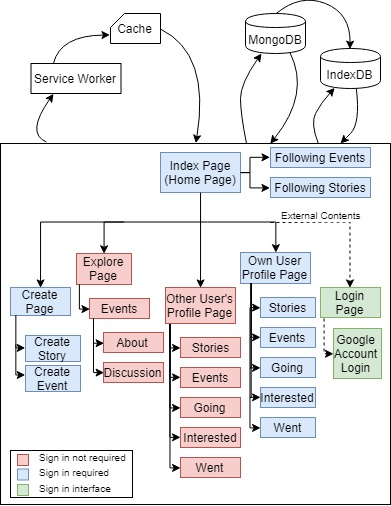
\includegraphics[width=8.5cm]{site_map.jpg}
    \caption{Demonstrates the flow of each web page in this PWA system along with the respective
    partial pages and external content pages.}
    \label{figure:site_map}
  \end{center}
\end{figure}
\begin{figure}[H]
  \begin{center}
    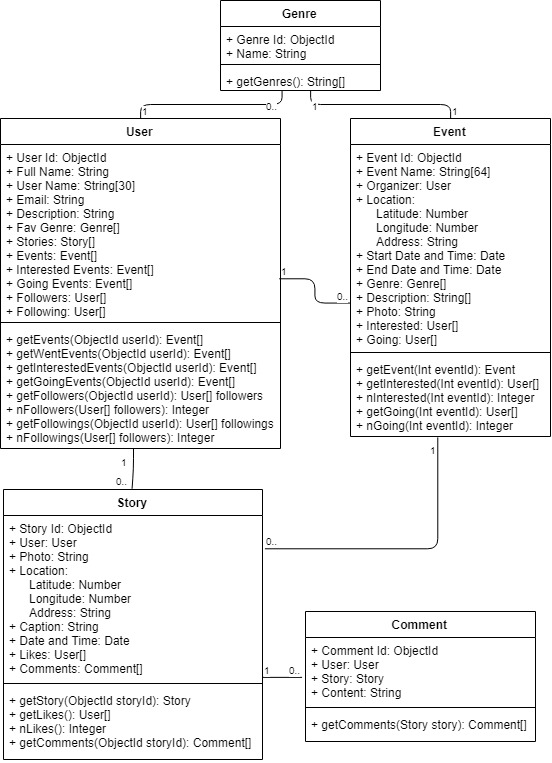
\includegraphics[width=15cm]{uml.jpg}
    \caption{Displays the structure of the database along with the types of content stored.}
    \label{figure:uml}
  \end{center}
\end{figure}

\end{document}
